\section{}
\[
H(s)=\frac{1}{s+1}\,.
\]
\subsection{Bode-Diagramm}
\begin{center}
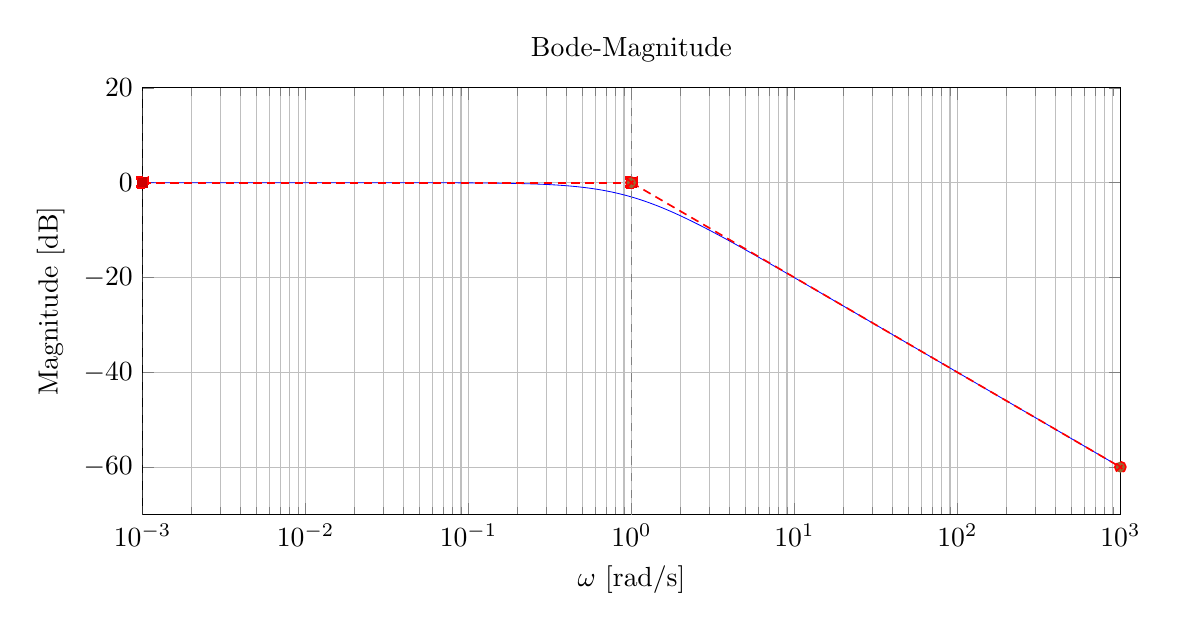
\begin{tikzpicture}
\begin{semilogxaxis}[
  width=14cm,height=7cm,
  ymin=-70,ymax=20,
  xmin=1e-3,xmax=1e3,
  xlabel={$\omega$ [rad/s]},
  ylabel={Magnitude [dB]},
  grid=both,
  title={Bode-Magnitude}
]
\addplot[
  domain=1e-3:1e3,
  samples=600,
  mark=none,
  line width=0.3pt,
  blue
] {-20*ln(sqrt(1 + x^2))/ln(10)};
\addplot+[domain=1e-3:1,samples=2,dashed,dash pattern=on 3pt off 2pt,line width=0.6pt,red] {0};
\addplot+[domain=1:1e3,samples=2,dashed,dash pattern=on 3pt off 2pt,line width=0.6pt,red] {-20*ln(x)/ln(10)};
\draw[gray,dashed] (rel axis cs:0,0) -- (rel axis cs:0,1);
\draw[gray,dashed] (axis cs:1,\pgfkeysvalueof{/pgfplots/ymin}) -- (axis cs:1,\pgfkeysvalueof{/pgfplots/ymax});
\node[gray,anchor=south east] at (axis cs:1,\pgfkeysvalueof{/pgfplots/ymax}) {\scriptsize Pol $\omega_p=1$};
\end{semilogxaxis}
\end{tikzpicture}
\vspace{6mm}
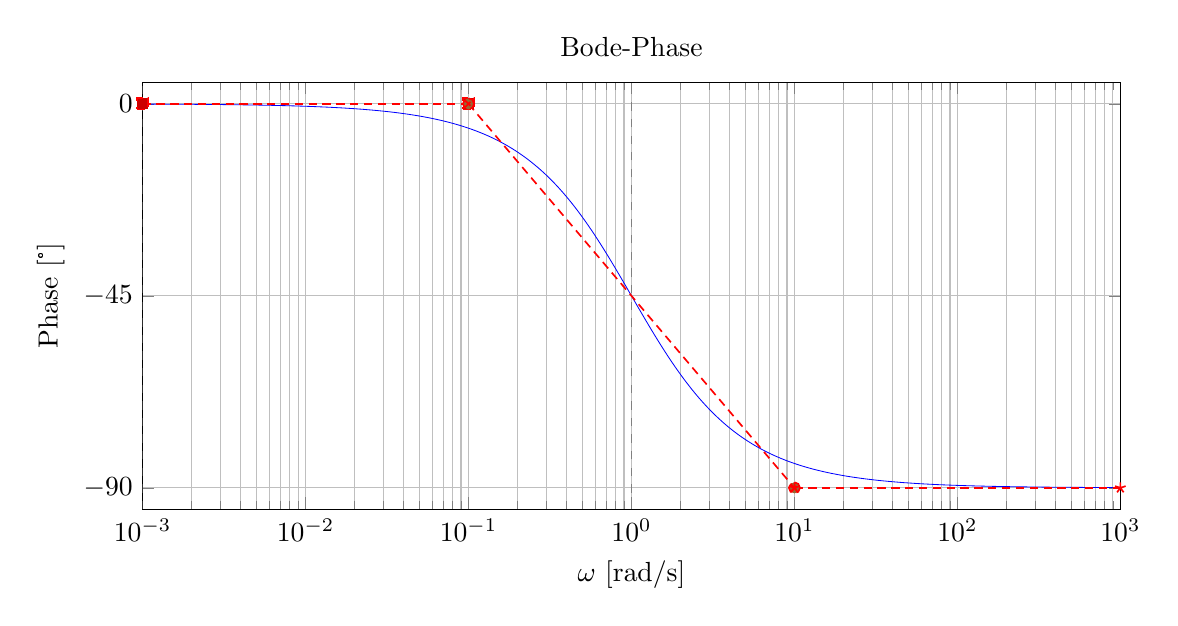
\begin{tikzpicture}
\begin{semilogxaxis}[
  width=14cm,height=7cm,
  xmin=1e-3,xmax=1e3,
  ymin=-95,ymax=5,
  ytick distance=45,
  xlabel={$\omega$ [rad/s]},
  ylabel={Phase [°]},
  grid=both,
  title={Bode-Phase}
]
\addplot[
  domain=1e-3:1e3,
  samples=600,
  mark=none,
  line width=0.3pt,
  blue
] {-atan(x)};
\addplot+[domain=1e-3:1e-1,samples=2,dashed,dash pattern=on 3pt off 2pt,line width=0.6pt,red] {0};
\addplot+[domain=1e-1:1e1,samples=2,dashed,dash pattern=on 3pt off 2pt,line width=0.6pt,red] {-45 - 45*ln(x)/ln(10)};
\addplot+[domain=1e1:1e3,samples=2,dashed,dash pattern=on 3pt off 2pt,line width=0.6pt,red] {-90};
\draw[gray,dashed] (rel axis cs:0,0) -- (rel axis cs:0,1);
\draw[gray,dashed] (axis cs:1,\pgfkeysvalueof{/pgfplots/ymin}) -- (axis cs:1,\pgfkeysvalueof{/pgfplots/ymax});
\node[gray,anchor=south east] at (axis cs:1,\pgfkeysvalueof{/pgfplots/ymax}) {\scriptsize Pol $\omega_p=1$};
\end{semilogxaxis}
\end{tikzpicture}
\end{center}
\newpage
\subsection{Erklärung}
\vspace{5mm}
\begin{description}[leftmargin=1.2em,labelsep=.6em,font=\bfseries]
\item[Schritt 1] DC-Faktor $1$: für $\omega\ll1$ ist $|H(\j\omega)|\approx1$; Betrag liegt bei $0\,\mathrm{dB}$ ohne Anfangssteigung, Phase $\approx0^\circ$.
\item[Schritt 2] Einfacher Pol bei $\omega_p=1\,\mathrm{rad/s}$: ab $\omega=1$ ändert die Magnituden-Steigung um $-20\,\mathrm{dB/dec}$; bei $\omega=1$ liegt die exakte Dämpfung bei $-10\log_{10}2\approx-3.01\,\mathrm{dB}$.
\item[Schritt 3] Grenzverhalten: für $\omega\gg1$ folgt $|H(\j\omega)|_{\mathrm{dB}}\approx-20\log_{10}\omega$; die Phase fällt in der Übergangsdekade $\omega_l=0.1\,\mathrm{rad/s}$ bis $\omega_h=10\,\mathrm{rad/s}$ von $0^\circ$ auf $-90^\circ$ (lineare Näherung: $-45^\circ-45\log_{10}\omega$ bei $\omega\in[0.1,10]$), mit $\angle H(\j\omega)= -45^\circ$ bei $\omega=1$.
\end{description}

\vspace{0.5cm}
\medskip
\noindent\textbf{Stückweise Näherung}
\[
|H(\j\omega)|_{\mathrm{dB}}\approx
\begin{cases}
0,& \omega\ll1,\\[4pt]
-10\log_{10}2,& \omega=1,\\[4pt]
-20\log_{10}\omega,& \omega\gg1,
\end{cases}
\qquad
\]
\newpage